%%%%%%%%%%%%%%%%%%%%%%%%%%%%%%%%%%%%%%%%%%%%%%%%%%%%%%%%%%%%%%%%%%%%%%%%%%%%%%%%
%% Title (en): Multiagent Systems and Organizations                           %%
%% Title (cs): Multiagentní systémy a organizace                              %%
%%                                                                            %%
%% Author: Bc. Lukáš Kúdela                                                   %%
%% Supervisor: Prof. RNDr. Petr Štěpánek, DrSc.                               %%
%%                                                                            %%
%% Academic year: 2011/2012                                                   %%
%%%%%%%%%%%%%%%%%%%%%%%%%%%%%%%%%%%%%%%%%%%%%%%%%%%%%%%%%%%%%%%%%%%%%%%%%%%%%%%%

% TODO Rename to Organization-Centric MAS Metamodels
\chapter{Modelling Organizations -- Existing Approaches}

In this chapter, we will introduce four approaches to modelling organizations in MASs.
All of them are based on platform-independent metamodels.

% PIM
In software engineering, \textit{platform-independent model} (PIM) is a model of a software system, that is independent of the specific technological platform used to implement it \cite{Wikipedia-PIM}.
% PIM - motivation
The main motivation to use a PIM is to build the model once and then automatically transform it to any number of platform-specific models (PSMs) for different (ALT: various) deployment platforms.

% PSM
The \textit{platform-specific model} (PSM) is a model of a software system bound to a specific technological platform (e.g. a hardware environment (processor), operating system or software environment (virtual machine)).
% PSM - motivation
Platform-specific models are indispensable for the actual implementation of a software system \cite{Wikipedia-PSM}

%%%%%%%%%%%%%%%%%%%%%%%%%%%%%%%%%%%%%%%%%%%%%%%%%%%%%%%%%%%%%%%%%%%%%%%%%%%%%%%%
\section{Models and Metamodels}

\subsection{Models and Modelling}

% Models, representation, conformance and modelling
Before talking about metamodels and metamodelling, its absolutely necessary to have a clear understanding of models, modelling and two basic relationships: representation and conformance. 

% Model - representation
A \textit{model} is a simplified \textit{representation} of a certain reality, for example, a system \cite{Genova09}.
A system can be represented by a set of different models.
Each model captures a specific aspect (or view) of the system depending on the purpose of that model.
A model must not represent the system with absolute preciseness; it is useful only because it is a simplified representation \cite{Genova09}.

% Model - conformance
A model also has to be expressed in some modelling language.
Therefore, the full definition of a model is the following: a model is a simplified representation of a certain reality \textit{conforming} to the rules of a certain modelling language \cite{Genova09}. In short, a model represents a system and conforms to a metamodel. Figure~\ref{figure:representation-and-conformance} illustrates both relationships.

% Figure: Representation and conformance relationships
\begin{figure}[h]
	\centering
	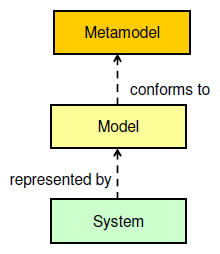
\includegraphics[width=0.25\textwidth]{images/representation-and-conformance-relationships.png}
	\caption{The representation and conformance relationships \cite{Genova09}}
	\label{figure:representation-and-conformance}
\end{figure}

% Modelling
Modelling, in the most general sense, is the use of a model to represent a certain reality for some cognitive purpose.

% Contextual substitutability
A model is characterized by \textit{contextual substitutability}: it should be able to answer a given set of questions in the same way the system would answer them \cite{Genova09}.

\subsection{Metamodels and Metamodelling}

% Metamodel
A metamodel is a special kind of model that specifies the abstract syntax of a modelling language \cite{OMG-MDA-Foundation-Model}.

% Metamodel - what it represents
A metamodel represents an abstract syntax of a modelling language; it does \textit{not} represent a model or a set of models
\footnote{The popular expression ``model of a model'' is particularly confusing.}.
% Metamodel - what it conforms to
A metamodel conforms to a meta-metamodel.

Consider the metalayers shown figure~\ref{figure:metalayers}:

% Figure: Metalayers
\begin{figure}[h]
	\centering
	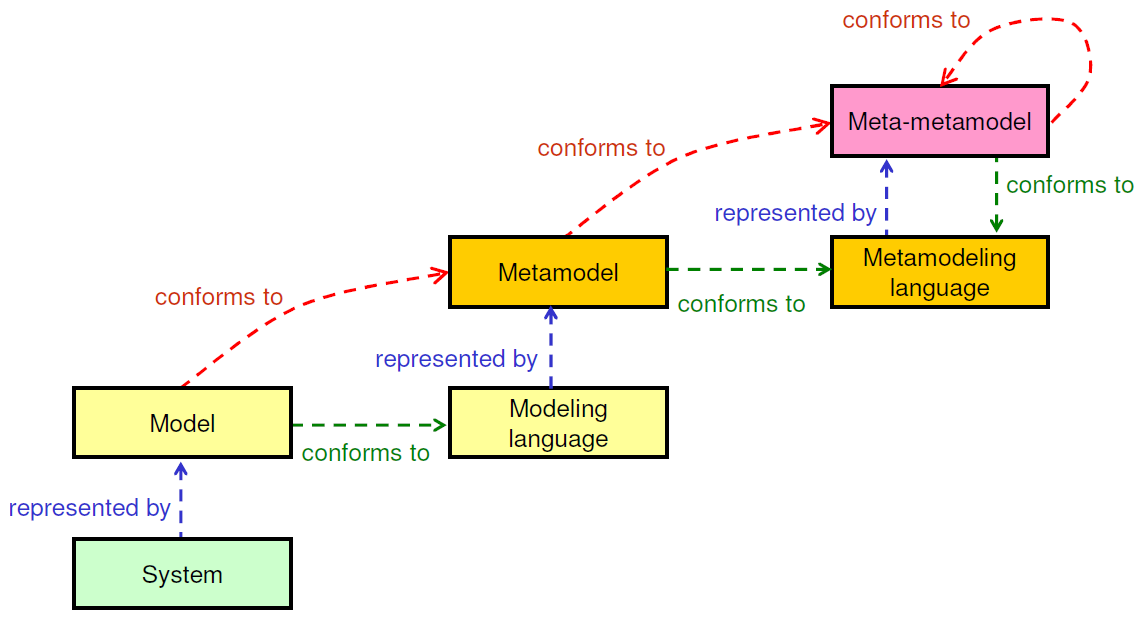
\includegraphics[width=0.75\textwidth]{images/metalayers.png}
	\caption{Metalayers \cite{Genova09}}
	\label{figure:metalayers}
\end{figure}

% Model conforms to metamodel
On the bottom level, a \textit{model} conforms to a modelling language whose abstract syntax is represented by a \textit{metamodel}.
Transitively, we can say that a \textit{model} conforms to a \textit{metamodel}.

On the middle level, a \textit{metamodel} conforms to a metamodelling language whose abstract syntax is represented by a \textit{meta-metamodel}.
Transitively, we can say that a \textit{metamodel} conforms to a \textit{meta-metamodel}.

On the top level, A \textit{reflexive meta-metamodel} conforms to a language whose abstract syntax is represented by \textit{itself}.
Transitively, we can say that a \textit{meta-metamodel} conforms to \textit{itself}.

% represented-by =/= conforms-to
The represented-by and conforms-to relationships are essentially different; arranging them in the same direction might be confusing.

% Using 'model' to refer to a metamodel
Since metamodels are models themselves, we will use the less cumbersome `model' to refer to a metamodel where it is obvious from the context that we are talking about the metamodel and not one of the models it specifies.  

%%%%%%%%%%%%%%%%%%%%%%%%%%%%%%%%%%%%%%%%%%%%%%%%%%%%%%%%%%%%%%%%%%%%%%%%%%%%%%%%
%% MASTER'S THESIS                                                            %%
%%                                                                            %% 
%% Title (en): Multi-Agent Systems and Organizations                          %%
%% Title (cs): Multiagentní systémy a organizace                              %%
%%                                                                            %%
%% Author: Bc. Lukáš Kúdela                                                   %%
%% Supervisor: Prof. RNDr. Petr Štěpánek, DrSc.                               %%
%%                                                                            %%
%% Academic year: 2011/2012                                                   %%
%%%%%%%%%%%%%%%%%%%%%%%%%%%%%%%%%%%%%%%%%%%%%%%%%%%%%%%%%%%%%%%%%%%%%%%%%%%%%%%%

\section{Aalaadin}

% Aallaadin - authors
This section introduces the \textit{Aalaadin} metamodel\footnote{\textit{Aalaadin} is the old name; the metamodel is now known as \textit{AGR} (for ``Agent, Group and Role''). We will use the fancier old name.} \cite{Ferber97}, \cite{Ferber98}, \cite{Ferber00} and \cite{Ferber03}, proposed in 1997 by Jacques Ferber, Oliver Gutknecht and their colleagues from Montpellier 2 University in Montpellier, France.
% Citation
The overview presented here is distilled from the seminal paper on \textit{Aalaadin} \cite{Ferber97}.

%% Aalaadin %%%%%%%%%%%%%%%%%%%%%%%%%%%%%%%%%%%%%%%%%%%%%%%%%%%%%%%%%%%%%%%%%%%%%

% Abstract organization vs. concrete organization
To understand the following text, it is essential to make a distinction between an \textit{abstract organization}\comments{FO} and a \textit{concrete organization}\comments{FO}.
An \textit{abstract organization} is the organization specification that exists in a MAS at design-time, whereas a \textit{concrete organization} is the actual organization that exists in a MAS at run-time.
Put differently, an abstract organization is a (possibly infinite) set of all imaginable organizations conforming to a common specification (sharing the same role structure) and a concrete organization is a member of this set.

% Organization type vs. organization token
Later we will use the terms \textit{organization type} and \textit{organization token} to refer to an abstract organization and a concrete organization respectively.
These terms try to capture the essence of the relationship between an abstract and concrete organization (namely, a concrete organization being an instance of an abstract organization and conversely, an abstract organization being a class of a concrete organization)

% Two models: concrete and abstract
The \textit{Aalaadin} metamodel comprises two models: \textit{Core model} and \textit{Methodological model}.

%%%%%%%%%%%%%%%%%%%%%%%%%%%%%%%%%%%%%%%%%%%%%%%%%%%%%%%%%%%%%%%%%%%%%%%%%%%%%%%%
\subsection{Core Model}

% Core model - about
The \textit{Core model} contains concepts for modelling concrete organizations, the so-called \textit{core} concepts: \textit{Agent}, \textit{Group} and \textit{Role}.
Figure~\ref{figure:aalaadin-core-model} illustrates the \textit{Core model}.

% Figure: Core model
\begin{figure}[h]
	\centering
	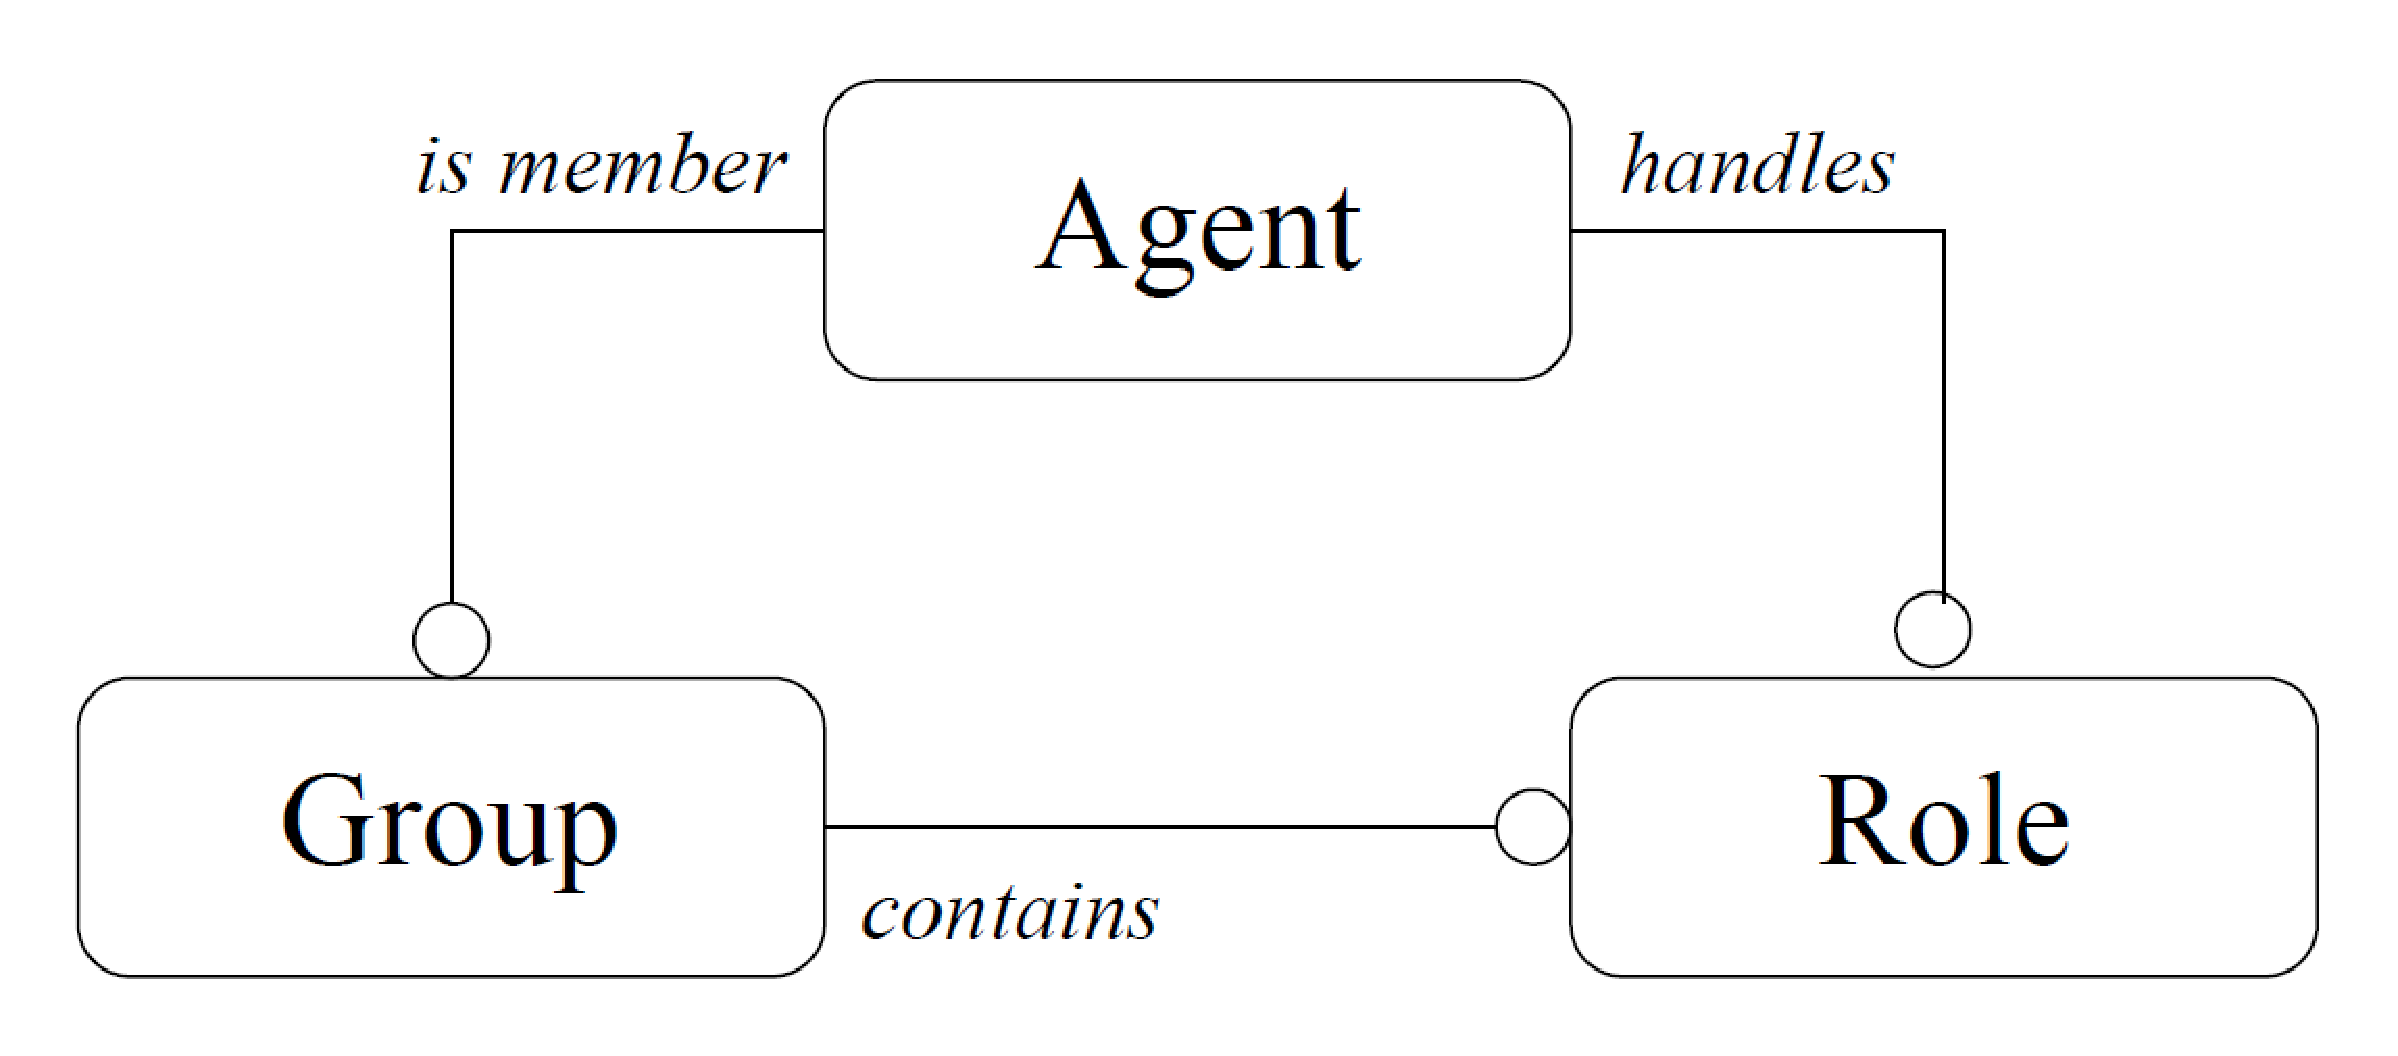
\includegraphics[width=0.4\textwidth]{images/aalaadin/core-model}
	\caption{The \textit{Core model} \cite{Ferber97}}
	\label{figure:aalaadin-core-model}
\end{figure}

\subsubsection*{Agent}

% Agent - definition
An \textit{agent} is defined in \cite{Ferber97} as an active communicating entity which plays roles within groups.

% Agent - no agent architecture imposed
\textit{Aalaadin} does not prescribe any particular agent architecture.
Indeed, any MAS metamodel striving for generality should impose as few constraints upon the resulting MAS models as possible.
After all, the decision of which agent architecture to employ is best made by the the MAS designer and relates to the MAS as such, not just its organizational structure.
As we will see, none of the metamodels introduced in this thesis force the MAS designer to adapt a concrete definition of agenthood.

\subsubsection*{Group}

% Group - definition
In \cite{Ferber97}, a \textit{group} is defined as atomic set of agent aggregation.
In its most basic form, a group is just a way to tag a set of agents, i.e. it has no structure.

% Group - characteristics
Groups have the following characteristics:
\begin{itemize}
	\item An agent can be a member of a number of groups simultaneously.
	This means that groups can overlap, which is major point of \textit{Aalaadin}.
	\item A new group can be founded by any agent; an agent must request its admission to an existing group.
	\item A group may be local or distributed across multiple machines.
\end{itemize}

The real advantage of grouping agents becomes apparent when we use roles to impose some structure to these groups.

\subsubsection*{Role}

% Role - definition
A \textit{role} is an abstract representation of an agent function, service or identification within a group \cite{Ferber97}.
An agent can play multiple roles, each of which is local to a particular group.
Similarly to group admission, playing a role in a group must be requested by the candidate agent (already a member of the group) and awarded by the group founder agent.

% Role & communication
In \textit{Aalaadin}, the communication is related to roles. Since an agent can play multiple roles, it can be engage in several independent dialogues simultaneously.

% Role - definition characteristics
The following characteristics are part of a role definition:
\begin{itemize}
	\item a \textit{uniqueness characteristic}---an indication whether the role is \textit{single} or \textit{multiple},
	\item a list of  \textit{competences}---conditions the candidate agent must satisfy to be eligible to play the role, and
	\item a list of \textit{capacities}---abilities attributed to an agent while it is playing the role.
\end{itemize}
A \textit{single role} can be played by at most one agent in a group, whereas a \textit{multiple role} can be played by any number of agents within a group.
By default a role is multiple, does not require any competences and does not provide any capacities.

% Group manager role
A special role in a group is the \textit{group manager} role, which is automatically granted to the group founder.
It has a competence to handle group membership and role playing requests.
It also has a capacity to revoke roles and cancel group membership.

%%%%%%%%%%%%%%%%%%%%%%%%%%%%%%%%%%%%%%%%%%%%%%%%%%%%%%%%%%%%%%%%%%%%%%%%%%%%%%%%
\subsection{Methodological Model}

% Methodological model - about
The \textit{Methodological model} contains concepts for modelling abstract organizations, the so-called \textit{methodological} concepts: \textit{Organization structure}, \textit{Group structure}, \textit{Interaction} and \textit{Agent class}.
These concepts are not present directly in concrete organizations, but only serve during the analysis and design phases.
Their purpose is to describe abstract organizations from which concrete organizations, described using the core concepts, will ultimately be derived.
Figure~\ref{figure:aalaadin-metamodel} shows the integrated \textit{Aalaadin} metamodel. The dotted ellipsis is the demarcation line between the \textit{Core model} and \textit{Methodological model}.

% Figure: Aalaadin metamodel
\begin{figure}[h]
	\centering
	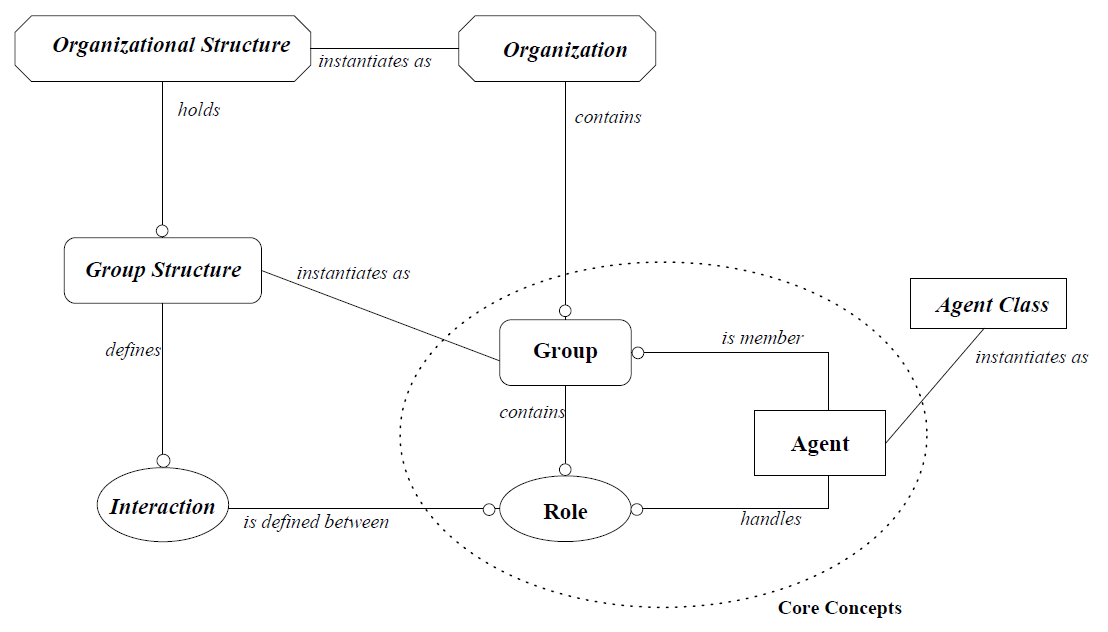
\includegraphics[width=\textwidth]{images/aalaadin/aalaadin-metamodel}
	\caption{The \textit{Aalaadin} metamodel \cite{Ferber97}}
	\label{figure:aalaadin-metamodel}
\end{figure}

\subsubsection*{Group Structure}

% Group structure - definition
A \textit{group structure} is an abstract description of a group \cite{Ferber97}.
It identifies all roles comprising the group and defines interactions among them.

% Group structure - definition characteristics
A group structure is defined by
\begin{itemize}
	\item a set of available roles that can be played by agents in the group, and
	\item a set of valid interaction schemes between the roles.
\end{itemize}

% Group structure - partial instantiation
Note that an actual group might be a partial instantiation of its defining group structure.
This means that during the MAS run, there might be a moment when some roles defined in the group structure are not played in an actual group.
This dynamic nature of groups allows for a great deal of run-time flexibility.

\subsubsection*{Organizational Structure}

% Organizational structure - definition
The \textit{organizational structure}, as defined in \cite{Ferber97}, is a set of group structures expressing the design of a multi-agent organization scheme.

% Organizational structure - about
The organizational structure can be seen as the specification of the problem to be solved (organization to be modelled) using a MAS.
Any sort of heterogeneity within a single system (e.g. agent architecture heterogeneity or language heterogeneity) can be managed by different group structures involved in the organizational structure.

% Organizational structure - partial instantiation
Similarly to groups, an asctual organization can be a incomplete manifestation of its defining organizational structure.
This means that while a MAS is running, there may be a point when some groups defined in the organizational structure are not present in an organization.
This also contributes to the overall run-time flexibility.

%%%%%%%%%%%%%%%%%%%%%%%%%%%%%%%%%%%%%%%%%%%%%%%%%%%%%%%%%%%%%%%%%%%%%%%%%%%%%%%%
\subsection{MadKit}

% MadKit - authors & references
The authors of \textit{Aalaadin} also developed an agent platform implementing their metamodel called \textit{MadKit}\footnote{Multi-Agent Development Kit ---\url{http://www.madkit.org/}} \cite{Ferber97}, \cite{Ferber98} and \cite{Gutknecht00}.

% MadKit - basic philosophy
The basic philosophy of the \textit{Aalaadin/MadKit} architecture is to use the platform itself for its own management wherever possible.
\textit{MadKit's} main design principles are \textit{micro-kernel architecture} and \textit{agentification of services}---all services except for the most fundamental ones provided by the micro-kernel are implemented as agents, organized in groups and identified by roles \cite{Ferber98}.

%%%%%%%%%%%%%%%%%%%%%%%%%%%%%%%%%%%%%%%%%%%%%%%%%%%%%%%%%%%%%%%%%%%%%%%%%%%%%%%%
%% MASTER'S THESIS                                                            %%
%%                                                                            %% 
%% Title (en): Multi-Agent Systems and Organizations                          %%
%% Title (cs): Multiagentní systémy a organizace                              %%
%%                                                                            %%
%% Author: Bc. Lukáš Kúdela                                                   %%
%% Supervisor: Prof. RNDr. Petr Štěpánek, DrSc.                               %%
%%                                                                            %%
%% Academic year: 2011/2012                                                   %%
%%%%%%%%%%%%%%%%%%%%%%%%%%%%%%%%%%%%%%%%%%%%%%%%%%%%%%%%%%%%%%%%%%%%%%%%%%%%%%%%

\section{O\&P}

% O&P - authors
This section introduces the \textit{O\&P} metamodel\footnote{The metamodel was not given a name by its authors. In this thesis, we will call it \textit{O\&P}.} \cite{Odell01}, \cite{Parunak02}, \cite{Odell03b}, \cite{Odell04b} and \cite{Odell05}, put forward in 2001 by James J. Odell, H. van Dyke Parunak and their colleagues.
% Citation
The overview presented here is extracted from the most complete paper on \textit{O\&P} \cite{Odell05}.

%% O&P %%%%%%%%%%%%%%%%%%%%%%%%%%%%%%%%%%%%%%%%%%%%%%%%%%%%%%%%%%%%%%%%%%%%%%%%%

%%%%%%%%%%%%%%%%%%%%%%%%%%%%%%%%%%%%%%%%%%%%%%%%%%%%%%%%%%%%%%%%%%%%%%%%%%%%%%%%
\subsection{Integrated Metamodel}

% Integrated model - about
Figure~\ref{figure:onp-metamodel} shows the integrated metamodel proposed in \cite{Odell05}.
The following subsections will focus on parts of the integrated metamodel that can be studied in isolation.
We present the full metamodel before discussing its parts so that the reader can follow the discussion knowing how each part fits into the big picture.

% Figure: O&P metmodel
\begin{figure}[ht]
	\centering
	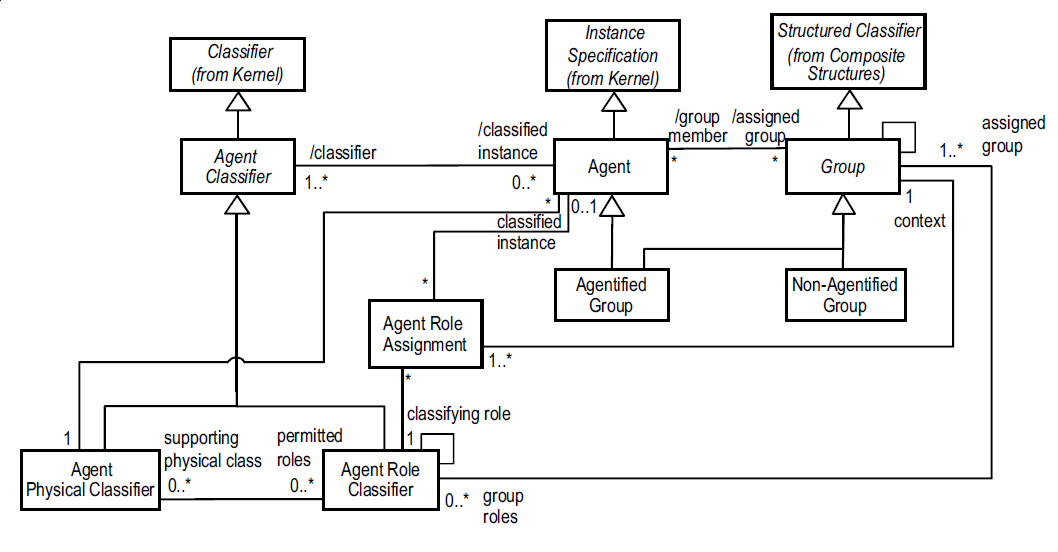
\includegraphics[width=\textwidth]{images/onp/onp-metamodel.png}
	\caption{The integrated \textit{O\&P} metamodel \cite{Odell05}}
	\label{figure:onp-metamodel}
\end{figure}

% UML Classifier vs. UML Class
To understand the integrated metamodel, it is essential to differentiate between the \textit{Classifier} and \textit{Class} UML classes.
In short, \textit{Classifier} does not have the features associated with a OOP class (e.g. the extended class, the list of implemented interfaces or attributes), while \textit{Class}, obviously, has them.
\textit{Class} is in fact a specialization of \textit{Classifier}.
It is important to make this distinction, because the agent classification is based on an extension of \textit{Classifier}, not \textit{Class}.
The reason for this is that the authors did not want to impose object-orientation upon their metamodel.
After all, it is not at all expected of an agent to exhibit behaviour intrinsic to an object, such as polymorphism.

%%%%%%%%%%%%%%%%%%%%%%%%%%%%%%%%%%%%%%%%%%%%%%%%%%%%%%%%%%%%%%%%%%%%%%%%%%%%%%%%
\subsection{Agent Classifiers and Agent Model}

\subsubsection*{Agent Classifier}

\textit{Agent Classifier} is a UML \textit{Classifier} that specifically provides a way to classify agent instances by a set of features that they have in common \cite{Odell05}.
Classification is important because it enables a common definition of a set of entities that are in some sense similar, i.e. share some features and/or capabilities.

Figure~\ref{figure:onp-agent-classifiers} shows \textit{Agent Classifier} and its two specializations: \textit{Agent Physical Classifier} and \textit{Agent Role Classifer}.

\begin{figure}[ht]
	\centering
	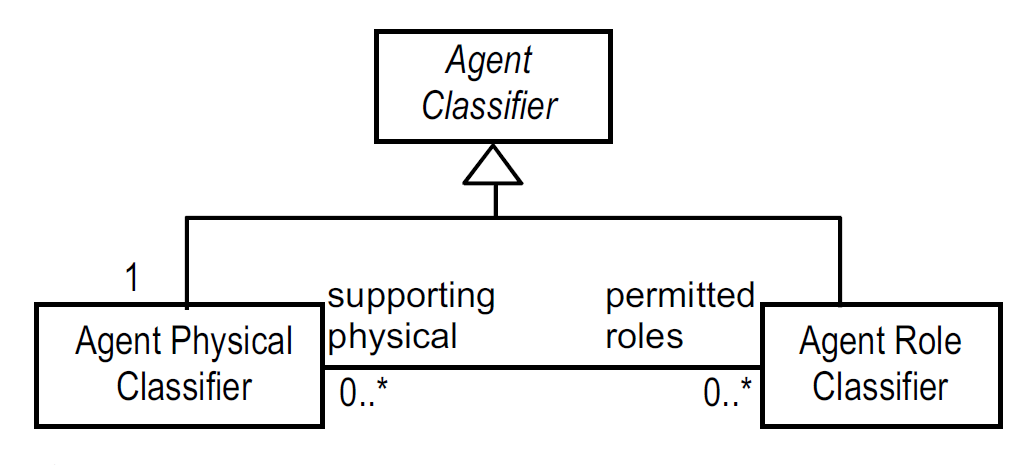
\includegraphics[width=0.6\textwidth]{images/onp/agent-classifiers.png}
	\caption{\textit{Agent Classifier} and its two specializations: \textit{Agent Physical Classifier} and \textit{Agent Role Classifier} \cite{Odell05}}
	\label{figure:onp-agent-classifiers}
\end{figure}

\subsubsection*{Agent Physical Classifier}

% Physical classifier - definition
The purpose of \textit{Agent Physical Classifier} is to define a set of features that an agent classified with it has independent of roles it plays \cite{Odell05}.
Every agent must be classified with exactly one physical classifier\footnote{Compare this with OOP, where every object must be an instance of exactly one class.} and is never reclassified during its lifetime.

% Physical classifiers vs. role classifiers
In contract to role classifiers, physical classifiers attribute primary and permanent features to agents.
Examples of physical classifiers from the real world are \textit{Human}, \textit{Male} or \textit{Female}.

Figure~\ref{figure:onp-physical-classifier-examples} shows some examples of physical classifiers forming a small class hierarchy.
Notice the \stereotype{agent physical classification} stereotype.

% Figure: Physical classifer examples
\begin{figure}[ht]
	\centering
	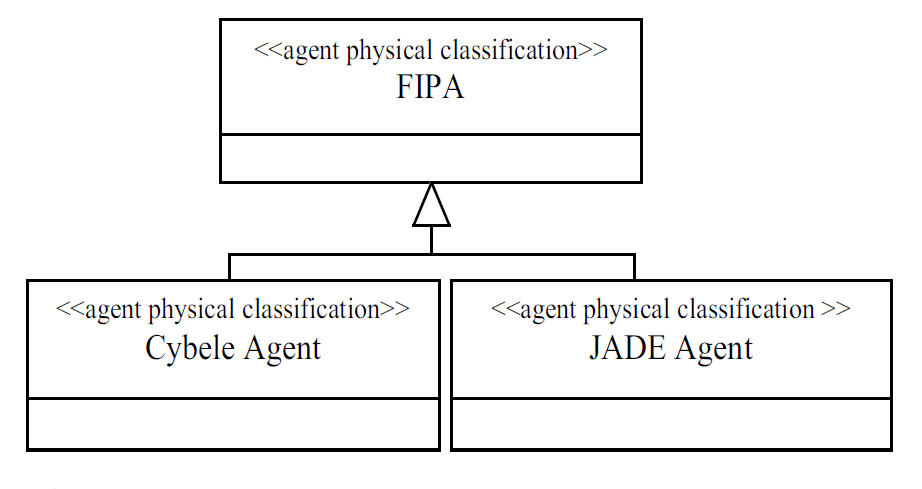
\includegraphics[width=0.5\textwidth]{images/onp/physical-classifier-examples.png}
	\caption{Examples of physical classifiers forming a class hierarchy \cite{Odell05}}
	\label{figure:onp-physical-classifier-examples}
\end{figure}

\subsubsection*{Agent Role Classifier}

% Role classifier - definition
\textit{Agent Role Classifier} is a classifier that defines a set of features that an agent classified with it acquires.
An agent can be classified with more than one role classifier at once (\textit{multiple classification}) and can be reclassified over time (\textit{dynamic classification}).

In comparison to physical classifiers, role classifiers ascribe secondary and transient features to agents.
An example of a role classifier from the real world would be \textit{Chess player}.

% Role hierarchy vs. class hierarchy
Figure~\ref{figure:onp-role-classifier-examples} depicts a small class hierarchy of role classifiers.
Notice the \stereotype{agent role} stereotype.

% Figure: Role classifer examples
\begin{figure}[ht]
	\centering
	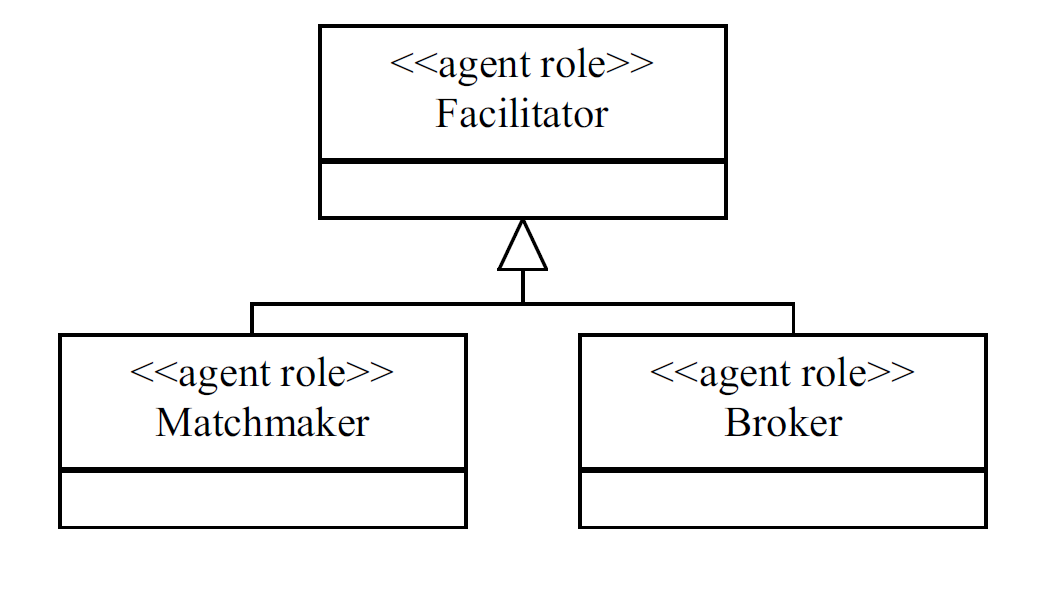
\includegraphics[width=0.5\textwidth]{images/onp/role-classifier-examples.png}
	\caption{Examples of role classifiers forming a class hierarchy \cite{Odell05}}
	\label{figure:onp-role-classifier-examples}
\end{figure}

\subsubsection*{Agent}

In \textit{O\&P}, the basic concepts are \textit{Agent Classifier} and \textit{Agent}.
These modelling constructs are considered fundamental, because they enable a MAS designer to model agents classes and agent instances respectively.
Agent classes are the design-time constructs providing the classification of the run-time constructs---agent instances.

\subsubsection*{Association between Agent Physical Classifier and Agent Role Classifier}

The association between \textit{Agent Physical Classifier} and \textit{Agent Role Classifier} specifies which role classifiers are permitted for each physical classifier, independent of the capabilities of the individual agents classified with that particular physical classifier \cite{Odell05}.

Figure~\ref{figure:onp-physical-classifier-role-classifier-association} illustrates this association.
It can be interpreted as follows. \textit{Jade} agents can play the \texttt{Broker} and \texttt{Manager} roles, and \textit{Cybele} agents can take on the role of \texttt{Broker}, \texttt{Trust Manager} and \texttt{Buyer}.

% Figure: Agent physical classifier <---> Agent role classifier association
\begin{figure}[ht]
	\centering
	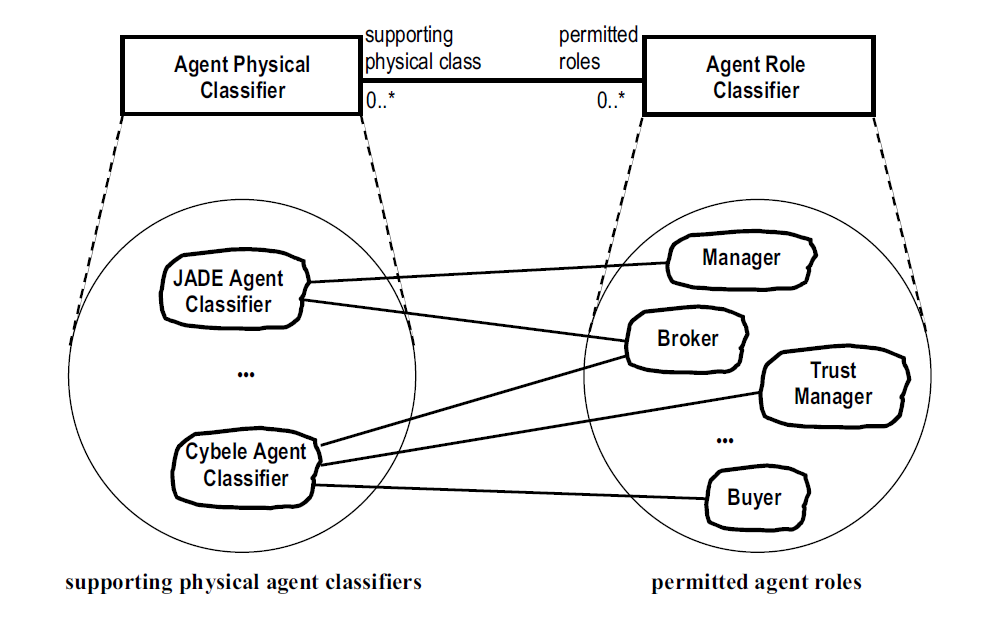
\includegraphics[width=0.8\textwidth]{images/onp/physical-classifier-role-classifier-association.png}
	\caption{The association between \textit{Agent Physical Classifier} and \textit{Agent Role Classifier} \cite{Odell05}}
	\label{figure:onp-physical-classifier-role-classifier-association}
\end{figure}

\subsubsection*{Association between Agent and Agent Classifier}

The association between \textit{Agent} and \textit{Agent Classifier} defines agents' features.
Each agent classifier classifies an agent as a member of a set of agents sharing some physical or role-related features.

% Physical vs. role classification
There are two main differences between the physical and role classification. First, the role classification is \textit{multiple} whereas the physical classification is \textit{single}.
While an agent can be classified with more than one (or even none) role classifiers at the same time, it must be classified with exactly one physical classifiers.
Second, the role classification is \textit{dynamic} in contrast to physical classification, which is \textit{static}.
Dynamic classification means that an agent can be declassified or reclassified with another role after the initial classification; static classification is invariant in time.

Figure~\ref{figure:onp-agent-agent-classifier-association} illuminates this association.
It can be read as follows. \texttt{Agent1}, a \textit{Jade} agent, is a \texttt{Manager}; \texttt{Agent2}, a \textit{Cybele} agent, is a \texttt{Manager} and \texttt{Buyer}; \texttt{Agent3}, another \textit{Cybele} agent, is a \texttt{Trust Manager}; and \texttt{Agent4}, also a \textit{Cybele} agent, is a \texttt{Broker}.

% Figure: Agent <---> Agent Classifier association
\begin{figure}[ht]
	\centering
	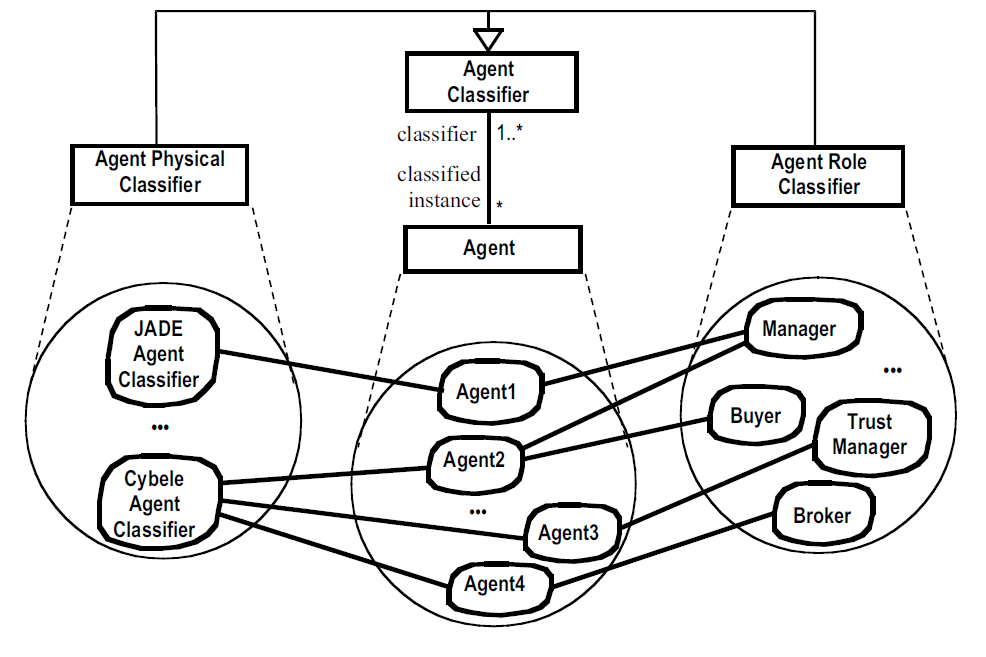
\includegraphics[width=0.8\textwidth]{images/onp/agent-agent-classifier-association.png}
	\caption{The association between \textit{Agent} and \textit{Agent Classifiers} \cite{Odell05}}
	\label{figure:onp-agent-agent-classifier-association}
\end{figure}

%%%%%%%%%%%%%%%%%%%%%%%%%%%%%%%%%%%%%%%%%%%%%%%%%%%%%%%%%%%%%%%%%%%%%%%%%%%%%%%%
\subsection{Group Model}

\subsubsection*{Group}

% Group - definition
A \textit{group} is a set of agents that are related via their roles, where these links must form
a connected graph within the group \cite{Odell05}.
This is the agent-centric way of lookig at a group.
Another way of to look at it is the role-centric way: a group is a composite structure consisting of interrelated roles, where each of the group's roles has a number of agent instances \cite{Odell05} playing that role.
A group can be formed to exploit the synergy of its members, resulting in an entity capable of performing operations that none of its constituents alone is capable of performing on its own.

Figure~\ref{figure:onp-group} shows the \textit{Group} class and its associations with \textit{Agent} and \textit{Role}.
The abstract \textit{Group} class extends the UML \textit{Structured Classifier}, which means that \textit{Group} is defined as composite structure\footnote{In UML, \textit{Structured Classifier} can be thought of as a structured set of classifiers. From this perspective, \textit{Group} is a structured set of \textit{Agent Role Classifiers}.}.

% Figure: Group
\begin{figure}[ht]
	\centering
	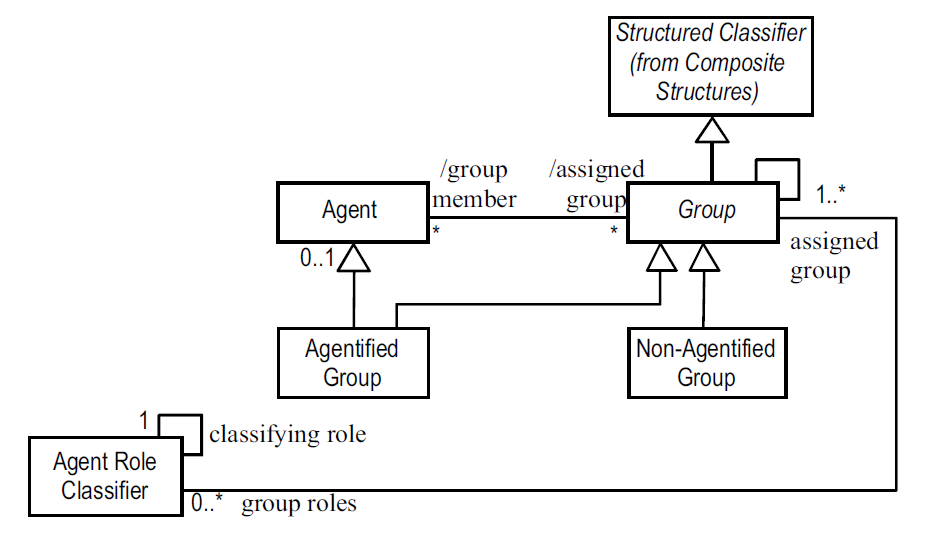
\includegraphics[width=0.8\textwidth]{images/onp/group.png}
	\caption{The \textit{Group} class and its associations \cite{Odell05}}
	\label{figure:onp-group}
\end{figure}

\subsubsection*{Association between Group and Agent}

% Association between Group and Agent
Conceptually, a group is constituted by a set of agents playing roles within that group.
The roles that the agents can play are represented by one or more agent role classifiers associated with this group.
Therefore, the set of agents forming a group can be derived from the group via the agent role classifiers \cite{Odell05}.

\subsubsection*{Association between Group and Role}

% Association between Group and Agent Role Classifier
Figure~\ref{figure:onp-group-role-association} illustrates the association between \textit{Group} and \textit{Role}.
Note that groups containing no roles are not allowed; each group must contain at least one role.
Also observe that each role has to be defined in at least one group, since roles only make sense within the context of a group.

% Figure: Group <---> Role association
\begin{figure}[ht]
	\centering
	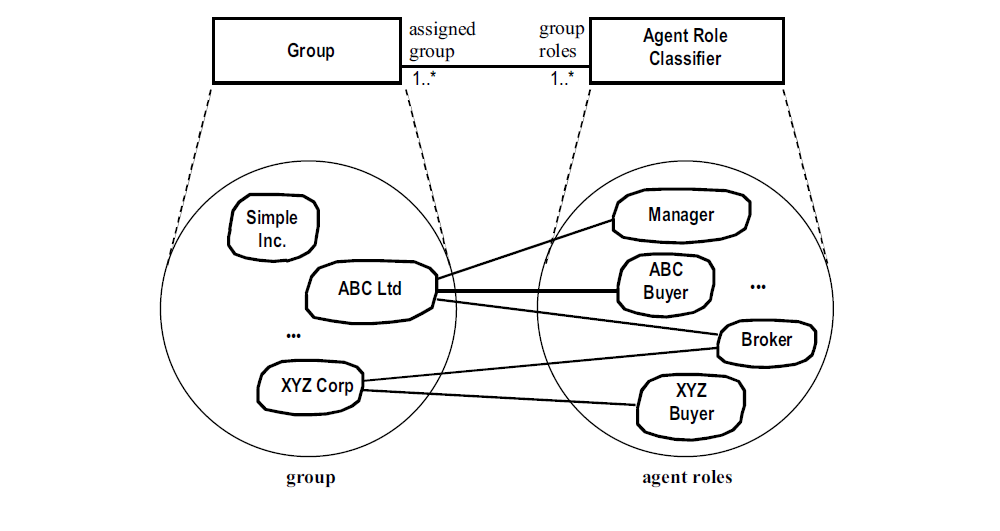
\includegraphics[width=0.8\textwidth]{images/onp/group-role-association.png}
	\caption{The association between \textit{Group} and \textit{Role} \cite{Odell05}}
	\label{figure:onp-group-role-association}
\end{figure}

\subsubsection*{Agentified and Non-Agentified Groups}

\textit{O\&P} differentiates between two types of groups: \textit{agentified}\comments{FO} and \textit{non-agentified}\comments{FO}.

% Agentified group
An \textit{agentified group} is a group that is also an agent in its own right, which means it has its own capability to interact \cite{Odell05}.
An agentified group can communicate with other agents (or agentified groups) directly, i.e. without a representative agent.
It can also be a member of other groups (agentified or not) and play roles like any other agent.
To achieve this in \textit{O\&P}, \textit{Agentified Group} is a subclass of both the \textit{Group} and \textit{Agent} classes.
Figure~\ref{figure:onp-agentified-group} shows an example of an agentified group.
Notice the \stereotype{agent} stereotype used to mark the group as agentified.

% Figure: agentified group
\begin{figure}[ht]
	\centering
	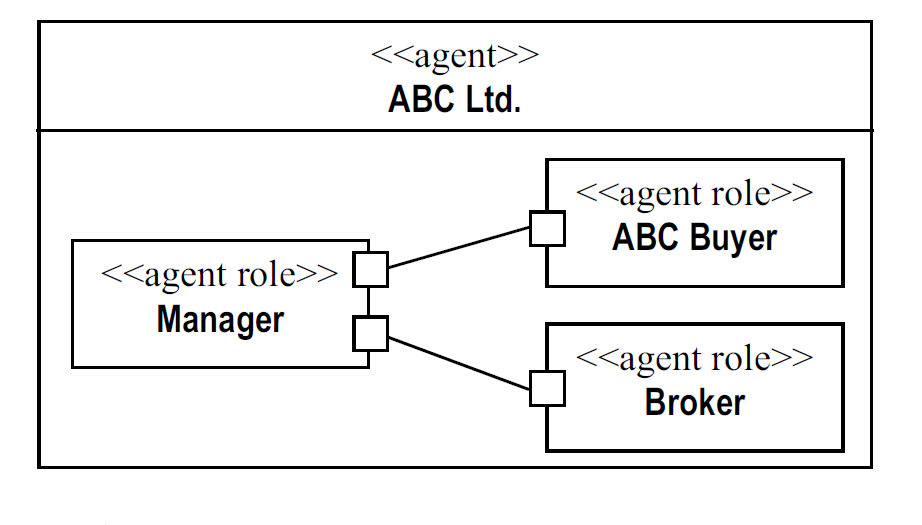
\includegraphics[width=0.5\textwidth]{images/onp/agentified-group.png}
	\caption{An example of an agentified group \cite{Odell05}}
	\label{figure:onp-agentified-group}
\end{figure}

% Non-agentified group
A \textit{non-agentified group}, while still being a first-class citizen, is not an agent in and of itself, meaning it has no capability to interact of its own.
A non-agentified group always communicates with other agents (including agentified groups) through one of its members acting as an intermediary.
This is achieved in \textit{O\&P} by \textit{Non-Agentified Group} subclassing only the \textit{Group} class and not the \textit{Agent} class.
An example of a non-agentified group is shown in figure~\ref{figure:onp-non-agentified-group}.
Notice the absence of the \stereotype{agent} stereotype.

% Figure: non-agentified group
\begin{figure}[ht]
	\centering
	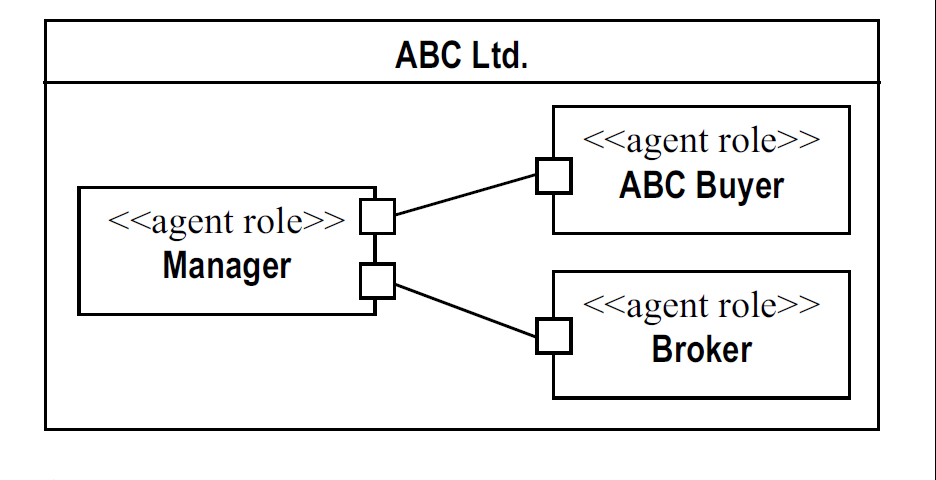
\includegraphics[width=0.5\textwidth]{images/onp/non-agentified-group.png}
	\caption{An example of a non-agentified group \cite{Odell05}}
	\label{figure:onp-non-agentified-group}
\end{figure}

%%%%%%%%%%%%%%%%%%%%%%%%%%%%%%%%%%%%%%%%%%%%%%%%%%%%%%%%%%%%%%%%%%%%%%%%%%%%%%%%
\subsection{Agent Role Assignment}

The assignment of roles to agents is dynamic, i.e. it changes in time, and is modelled by \textit{Agent Role Assignment}.
Figure~\ref{figure:onp-agent-role-assignment} shows the \textit{Agent Role Assignment} class and its associations.

% Figure: Agent Role Assignment class
\begin{figure}[ht]
	\centering
	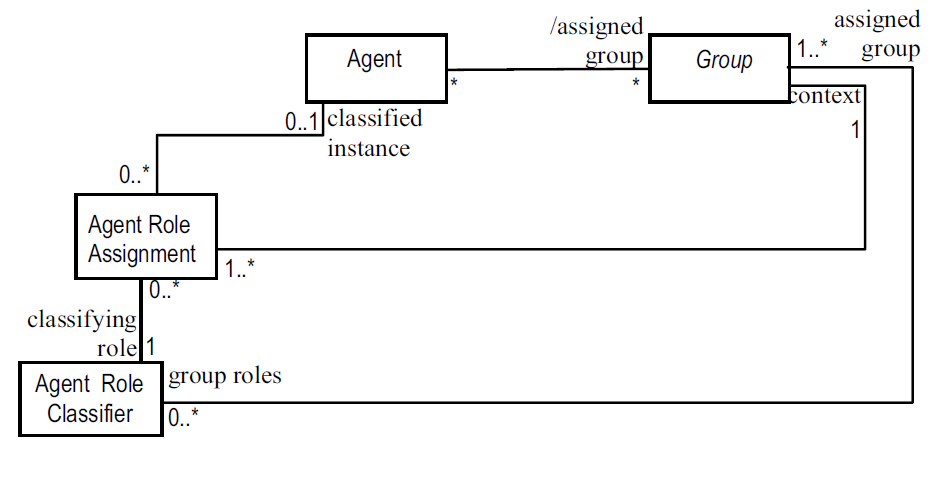
\includegraphics[width=0.8\textwidth]{images/onp/agent-role-assignment.png}
	\caption{The \textit{Agent Role Assignment} class and its associations \cite{Odell05}}
	\label{figure:onp-agent-role-assignment}
\end{figure}

\subsubsection*{Agent Role Assignment as a Ternary Association}

A model with a direct association between \textit{Agent} and \textit{Agent Role Classifier} could represent agents playing roles.
However, such model would not be able to represent a situation where an agent plays a role in one group but does not play it in another.
To model this kind of situation, it is necessary to augment the agent-to-role association with a group context.
This yields a ternary association, reified\footnote{\textit{Reification} is the process of turning an implicit abstract idea about some concept into an explicit concrete model of that concept.} in \textit{O\&P} as the \textit{Agent Role Assignment} class, whose instances link an agent to a role in a group.

\subsubsection*{Position}

It is possible to associate a group with a role leaving an agent unspecified.
Such association is called a \textit{position} and represents a situation where a concrete agent playing a role within a particular group is yet to be determined.
This turns out to be an extremely useful modelling concept, since more often than not, the organization modeller does not know (or simply does not care) which agent will actually take a particular position when the MAS is run.
Unfortunately, this association is not reified in \textit{O\&P}.
If it was reified as the \textit{Position} class, the \textit{Agent Role Assignment} class could be viewed as a reified association between the \textit{Position} and \textit{Agent} classes.

%%%%%%%%%%%%%%%%%%%%%%%%%%%%%%%%%%%%%%%%%%%%%%%%%%%%%%%%%%%%%%%%%%%%%%%%%%%%%%%%
%% MASTER'S THESIS                                                            %%
%%                                                                            %% 
%% Title (en): Multi-Agent Systems and Organizations                          %%
%% Title (cs): Multiagentní systémy a organizace                              %%
%%                                                                            %%
%% Author: Bc. Lukáš Kúdela                                                   %%
%% Supervisor: Prof. RNDr. Petr Štěpánek, DrSc.                               %%
%%                                                                            %%
%% Academic year: 2011/2012                                                   %%
%%%%%%%%%%%%%%%%%%%%%%%%%%%%%%%%%%%%%%%%%%%%%%%%%%%%%%%%%%%%%%%%%%%%%%%%%%%%%%%%

\section{PIM4Agents}

% PIM4Agents - authors
This section introduces the PIM4Agents metamodel\footnote{For ``Platform-independent model for agents''.} \cite{Hahn07a}, \cite{Hahn07b} and \cite{Hahn08} proposed in 2007 by Christian Hahn, Cristián Madrigal-Mora and Klaus Fischer from German Research Centre for Artificial Intelligence (Deutsches Forschungszentrum f\"{u}r K\"{u}nstliche Intelligenz, DFKI).

% Citation
We will present only a brief overview (distilled from \cite{Hahn07b}) since our work does not draw much inspiration from PIM4Agents.

%% PIM4Agents %%%%%%%%%%%%%%%%%%%%%%%%%%%%%%%%%%%%%%%%%%%%%%%%%%%%%%%%%%%%%%%%%%

% PIM4Agents & MDA
PIM4Agents has been specifically designed to be employed in the Model-driven engineering (MDE) software development methodology, more precisely in Model-driven architecture (MDA) by Object Management Group (OMG).
Apart from the platform-independent metamodel itself, the authors have proposed two platform-specific metamodels: JackMM and JadeMM for the JACK and Jade agent platforms respectively.
They have also described two sets of model transformations to convert PIMs to PSMs: PIM4Agents-to-JackMM and PIM4Agents-to-JadeMM.

%%%%%%%%%%%%%%%%%%%%%%%%%%%%%%%%%%%%%%%%%%%%%%%%%%%%%%%%%%%%%%%%%%%%%%%%%%%%%%%%
\subsection*{Core Model}

% Core metamodel
To support adaptability, PIM4Agents is structured around a small core that could be augmented with extensions to model specific aspects of MASs, for example, security.
Figure~\ref{figure:pim4agents-metamodel} shows the core model.

% Agent
The metamodel, like previously introduced metamodels, is built around the concept of \textit{Agent}, an autonomous entity capable of sensing its environment and acting upon it.
Each \textit{Agent} has access to a set of \textit{Resources} from its surrounding \textit{Environment} \cite{Hahn07b}.

% Behaviour, Capability
A \textit{Behaviour} can be atomic or composed of sub-behaviours.
This way, a whole hierarchy of specific \textit{Behaviours} can be created.
A \textit{Behaviour} may also send or receive \textit{Messages} according to a \textit{Protocol}.
A \textit{Capability} allows to group conceptually related \textit{Behaviours} \cite{Hahn07b}.

% Role, Cooperation, Protocol, Message
A \textit{Role} is an abstraction of the social behaviour of an \textit{Agent} in a given social context, usually a \textit{Cooperation}; it specifies the responsibilities of a \textit{Agent} in that social context.
A \textit{Cooperation} represents the interaction between \textsc{Agents} playing the required set of \textit{Roles}.
The detailed realisation of this interaction is described by a \textit{Protocol} that specifies the \textit{Messages} exchanged between the \textit{Roles} and at which point in time they are to be expected.
A \textit{Protocol} is executed by a set of \textit{Behaviours} sending and receiving \textit{Messages} in accordance to their \textit{Roles}.

% Organziation
\textit{Agents} can take part in an \textit{Organization}, a special kind of \textit{Cooperation} that also has the same characteristics as an \textit{Agent}.
Being a \textit{Cooperation}, an \textit{Organization} can have its own internal protocol that specifies how it coordinates its members.
Being also an \textit{Agent}, an \textit{Organization} can play roles in other \textit{Organizations} (super-organization) and has \textit{Capabilities} which can be performed by its members, be they \textit{Agents} or other \textit{Organizations} (sub-organizations).

% Figure: PIM4Agents metamodel
\begin{figure}[ht]
	\centering
	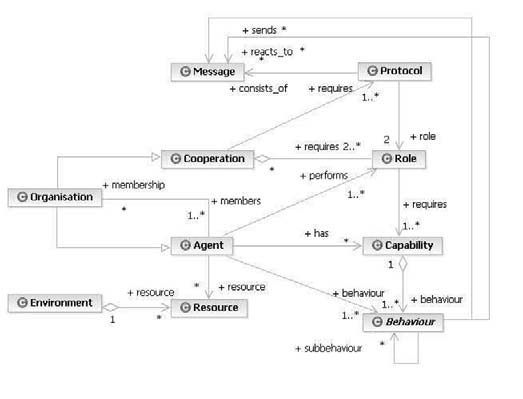
\includegraphics[width=0.6\textwidth]{images/pim4agents/pim4agents-metamodel.png}
	\caption{The PIM4Agents core model \cite{Hahn07b}}
	\label{figure:pim4agents-metamodel}
\end{figure}

%%%%%%%%%%%%%%%%%%%%%%%%%%%%%%%%%%%%%%%%%%%%%%%%%%%%%%%%%%%%%%%%%%%%%%%%%%%%%%%%
\subsection{JadeOrgs}

JadeOrgs
\cite{Madrigal-Mora08} and \cite{Madrigal-Mora09}
is an extension of the Jade framework that implements the JadeMM platform-specific metamodel.

JadeMM is defined using Eclipse Modeling Framework (EMF) to exploit EMF's code generation facility.
Given a platform-independent model of a MAS (conforming to PIM4Agents), the corresponding Jade/JadeOrgs platform-specific model (conforming to JadeMM) can be derived automatically.

%%%%%%%%%%%%%%%%%%%%%%%%%%%%%%%%%%%%%%%%%%%%%%%%%%%%%%%%%%%%%%%%%%%%%%%%%%%%%%%%
%% Title (en): Multiagent Systems and Organizations                           %%
%% Title (cs): Multiagentní systémy a organizace                              %%
%%                                                                            %%
%% Author: Bc. Lukáš Kúdela                                                   %%
%% Supervisor: Prof. RNDr. Petr Štěpánek, DrSc.                               %%
%%                                                                            %%
%% Academic year: 2011/2012                                                   %%
%%%%%%%%%%%%%%%%%%%%%%%%%%%%%%%%%%%%%%%%%%%%%%%%%%%%%%%%%%%%%%%%%%%%%%%%%%%%%%%%

\section{powerJade}

% powerJade - authors
This section introduces the powerJade metamodel
\footnote{The name is intentionally uncapitalized.}
\cite{Baldoni08a}, \cite{Baldoni08b}, \cite{Baldoni09} and \cite{Baldoni10}
put forward in 2008 by Matteo Baldoni, Guido Boella and their colleagues from University of Turin in Turin, Italy.

% Citation
The overview presented here is extracted from the most complete paper on powerJade \cite{Baldoni10}.

%% Summary %%%%%%%%%%%%%%%%%%%%%%%%%%%%%%%%%%%%%%%%%%%%%%%%%%%%%%%%%%%%%%%%%%%%%

% powerJade inspired by powerJava
powerJade is inspired by the authors' previous work on powerJava -- an extension of the Java programming language with an explicit role construct, based on an ontological analysis of roles described in \cite{Baldoni05}, \cite{Baldoni06a}, \cite{Baldoni06b} and \cite{Baldoni07}.

% Definitions (organization, role)
An organization belongs to the social reality and it can only be interacted with via the roles it defines \cite{Boella06}.
Specifically, it is not an object that could be manipulated from outside like objects in OOP.
The concept of organization is useful not only when modelling problem domains including organizations of some kind.
Indeed, we can view every object as an organization offering different ways of interacting with it, each represented by a different role.

%%%%%%%%%%%%%%%%%%%%%%%%%%%%%%%%%%%%%%%%%%%%%%%%%%%%%%%%%%%%%%%%%%%%%%%%%%%%%%%%
\subsection*{Organizational Structure Metamodel}

An ontological analysis of roles in \cite{Boella04} yields the following properties of roles:
\begin{itemize}
	\item \textit{Foundation} -- A role instance is always associated with an instance of the organization class to which is belongs and with a player instance.
	\item \textit{Definitional dependence} -- The definition of a role depends on the organizations it belongs to.
	\item \textit{Institutional powers} -- Role operations (called \textit{powers}) have access to the state of the organization and other roles of the organization.
	\item \textit{Prerequisities} -- To be granted a role, the player must be able to perform operations (called \textit{requirements}) which can be requested while it plays the role.
\end{itemize}


The metmodel in \cite{Boella04} is focused on organizational structure.
% Ontological status of organizations and roles compared to agents
The ontological status of organizations and roles does not differ completely from that of agents or even objects \cite{Boella04}.
% Differences
On one hand, organizations and roles, unlike agents, are not autonomous and act via their members and players.
Additionally, roles, unlike objects, do not exist as independent entities, since they are necessarily linked to organizations.
% Similarities
On the other hand, organizations and roles, like agents, are descriptions of complex behaviour.
In the real world, organizations are considered legal entities; they can even act like agents, albeit via a representative role.
Since they share some properties with agents, they can be modelled using similar primitives.

%%%%%%%%%%%%%%%%%%%%%%%%%%%%%%%%%%%%%%%%%%%%%%%%%%%%%%%%%%%%%%%%%%%%%%%%%%%%%%%%
\subsection*{Role Dynamics Metamodel}

The metamodel in \cite{Dastani04} is focused on role dynamics.
% Four operations: Enact, deact, actiavte, deactivate
Four operations pertaining to the role dynamics are defined: \textit{enact} and \textit{deact} meaning that an agent acquires and relinquishes a role, and \textit{activate} and \textit{deactivate} meaning that the agent actually starts and stops playing a role.
Even though it is possible (and very common) for an agent to be enacting multiple roles simultaneously, only one of these can be active at any moment.
Naturally, it is possible that at some moment none is active.
In particular, when an agent is invoking a power, exactly one of its roles is active.

%%%%%%%%%%%%%%%%%%%%%%%%%%%%%%%%%%%%%%%%%%%%%%%%%%%%%%%%%%%%%%%%%%%%%%%%%%%%%%%%
\subsection*{Unified Metamodel}

The authors of powerJade merged the models in \cite{Boella04} (organization strucure) and \cite{Boella04} (role dynamics) into a unified metamodel.
Organizations and roles are not just design-time abstractions with no run-time projections and players are not just isolated agents; they are all agents interacting with one another.
A logical specification of this unified metamodel can be found in \cite{Boella07}.

%%%%%%%%%%%%%%%%%%%%%%%%%%%%%%%%%%%%%%%%%%%%%%%%%%%%%%%%%%%%%%%%%%%%%%%%%%%%%%%%
\subsection*{Powers and Requirements}

% Role (AOPwO) vs. interace (OOP)
Roles in powerJade can be compared to interfaces from OOP.
Just like an interface is a contract between a calling class and called class, a role is a contract between an organization and an agent.

% OOP: called class implements interfaces vs. powerJade: player enacts roles
% OOP
In OOP, the relationship between a class and the interfaces it implements is a rigid one -- the interfaces a class implements are part of its design-time definition and cannot be implemented or un-implemented at run-time.
% powerJade
In contrast, the relationship between a player and roles it enacts in powerJade is a flexible one -- the roles the a player enacts are not part of its design-time definition and can be enacted and deacted at run-time.

% OOP: interfaces declare methods & events vs. AOPwO: roles define requirements & powers
% OOP
Interfaces in OOP declare methods and events.
When implementing an interface, a class has to implement its methods and it can raise its events.
% powerJade
Similarly, roles in powerJade define \textit{requirements} and \textit{powers}.
When eancting a role, a player has to execute its requirements and it can invoke its powers.
Thus, interface methods correspond to role requirements (both are responsibilities), while interface events are analogous to role powers (both are competences).